%%%%%%%%%%%%%%%%%%%%%%%%%%%%%%%%%%%%%%%%%%%%%%%%%%%%%%%%%%%%%%%%%%%%%
%%                                                                 %%
%% Please do not use \input{...} to include other tex files.       %%
%% Submit your LaTeX manuscript as one .tex document.              %%
%%                                                                 %%
%% All additional figures and files should be attached             %%
%% separately and not embedded https://pt.overleaf.com/project/621fb3a13d703216d2e84009in the \TeX\ document itself.       %%
%%                                                                 %%
%%%%%%%%%%%%%%%%%%%%%%%%%%%%%%%%%%%%%%%%%%%%%%%%%%%%%%%%%%%%%%%%%%%%%
%%\documentclass[referee,sn-basic]{sn-jnl}% referee option is meant for double line spacing

%%=======================================================%%
%% to print line numbers in the margin use lineno option %%
%%=======================================================%%

%%\documentclass[lineno,sn-basic]{sn-jnl}% Basic Springer Nature Reference Style/Chemistry Reference Style

%%======================================================%%
%% to compile with pdflatex/xelatex use pdflatex option %%
%%======================================================%%

%%\documentclass[pdflatex,sn-basic]{sn-jnl}% Basic Springer Nature Reference Style/Chemistry Reference Style

%%\documentclass[sn-basic]{sn-jnl}% Basic Springer Nature Reference Style/Chemistry Reference Style
\documentclass[pdflatex,sn-mathphys,lineno]{sn-jnl}% Math and Physical Sciences Reference Style

%%%% Standard Packages
%%<additional latex packages if required can be included here>
%%%%
\jyear{2021}%

%% as per the requirement new theorem styles can be included as shown below
\theoremstyle{thmstyleone}%
\newtheorem{theorem}{Theorem}%  meant for continuous numbers
%%\newtheorem{theorem}{Theorem}[section]% meant for sectionwise numbers
%% optional argument [theorem] produces theorem numbering sequence instead of independent numbers for Proposition
\newtheorem{proposition}[theorem]{Proposition}% 
%%\newtheorem{proposition}{Proposition}% to get separate numbers for theorem and proposition etc.

\theoremstyle{thmstyletwo}%
\newtheorem{example}{Example}%
\newtheorem{remark}{Remark}%

\theoremstyle{thmstylethree}%
\newtheorem{definition}{Definition}%

\raggedbottom
%%\unnumbered% uncomment this for unnumbered level heads

\begin{document}

\title[Comparison of Home Location Estimation Methods using Smartphone GPS Data]{Comparison of Home Location Estimation Methods using Smartphone GPS Data}

\author[1]{\fnm{Rajat} \sur{Verma}}
\author[1]{\fnm{Zengxiang} \sur{Lei}}
\author[1]{\fnm{Shagun} \sur{Mittal}}
\author[1]{\fnm{Xiaowei} \sur{Chen}}
%\equalcont{These authors contributed equally to this work.}

\author*[1]{\fnm{Satish V.} \sur{Ukkusuri}}\email{sukkusur@purdue.edu}

\affil*[1]{\orgdiv{Lyles School of Civil Engineering}, \orgname{Purdue University}, \orgaddress{\street{550 Stadium Mall Avenue}, \city{West Lafayette}, \postcode{47907}, \state{Indiana}, \country{USA}}}

\abstract{
Estimation of a person’s most prominent location (MPL), such as home or work location, from large-scale location-based services (LBS) data from smartphones is a common task in many applications in quantitative human mobility assessment. However, commonly used  MPL detection methods are often arbitrary and unexamined. In this study, we compare \#\# MPL detection algorithms on high-quality LBS data using a few performance metrics. We discuss the conceptual and empirical differences between these methods and comment on their use cases. We find that … method works the best when …. Our results will be helpful for human mobility analysis tasks such as …
}

\keywords{GPS, cell phone data, home location, data inference}

\maketitle

\section{Introduction}\label{sec1}
% Background
MPL detection plays an essential role in many () studies such as (). Details about the role.

% Challenges and research gaps
Despite its significance, little attention has been paid on ensuring the reliability of the estimated MPLs. In literature, researchers often state their MPL detection methods plainly without thorough validation, resulting in doubts about the validity of the subsequent findings based on the estimated MPLs.

In this paper, we do ... Study Overview. Our contributions are three-fold:

\begin{enumerate}
    \item Contrib 1
    \item Contrib 2
    \item Contrib 3
\end{enumerate}

The rest of this paper is organized as follows. Section 2. Section 3. Section 4. Section 5.

\begin{figure}[ht]
    \centering
    \includegraphics[width=0.8\textwidth]{figures/Study overview.png}
    \caption{Study overview}
    \label{fig:my_label1}
\end{figure}

\subsection{Related work}

In this section, we review different home location detection algorithms and their applications.

\begin{itemize}
    \item Shen et al. (2014) summarized the different types of home detection algorithms \cite{Shen2014}.
\end{itemize}

% We should directly go with the study design, the GPS data description can be put in the Result section
\section{Data and methods}

\subsection{GPS data description}
This is the section for the GPS data description.

\subsubsection{Data filtering}
\begin{figure}[ht]
    \centering
    \includegraphics[width=0.8\textwidth]{figures/Selecting users.png}
    \caption{Selecting users}
    \label{fig:my_label2}
\end{figure}

\subsection{Performance metrics}

\subsubsection{Residential detection rate}

\subsubsection{Proximity to daily data}
% Definition
This metric makes use of the idea that a home location should be the origin/destination of one’s daily trips. Given a person’s identified “home location” and observed trajectories (i.e., a sequence of coordinates), we calculate the distance between the “home location” and trajectory  for each day, then take the average of these distances as its proximity to daily data.

% A small example
The following figure (to be added) shows an example of how to obtain this metric. In the example, there are two candidate home locations: a red dot and a green cross.  The red one only falls on the trajectory of day 1 and is far away from the trajectories for other days. In this case, the conjecture is that a red dot is just a place where this person hung out during day 0’s evening and the green cross is more likely to be his/her home location.

% More implication
This metric, not only can be used to compare different MPL detection methods but can also serve as a data cleaning criterion: if no point is found to have low proximity to daily data, this means we are unlikely to identify the home location and we may remove this person’s data from the analyses.

\begin{figure}[ht]
    \centering
    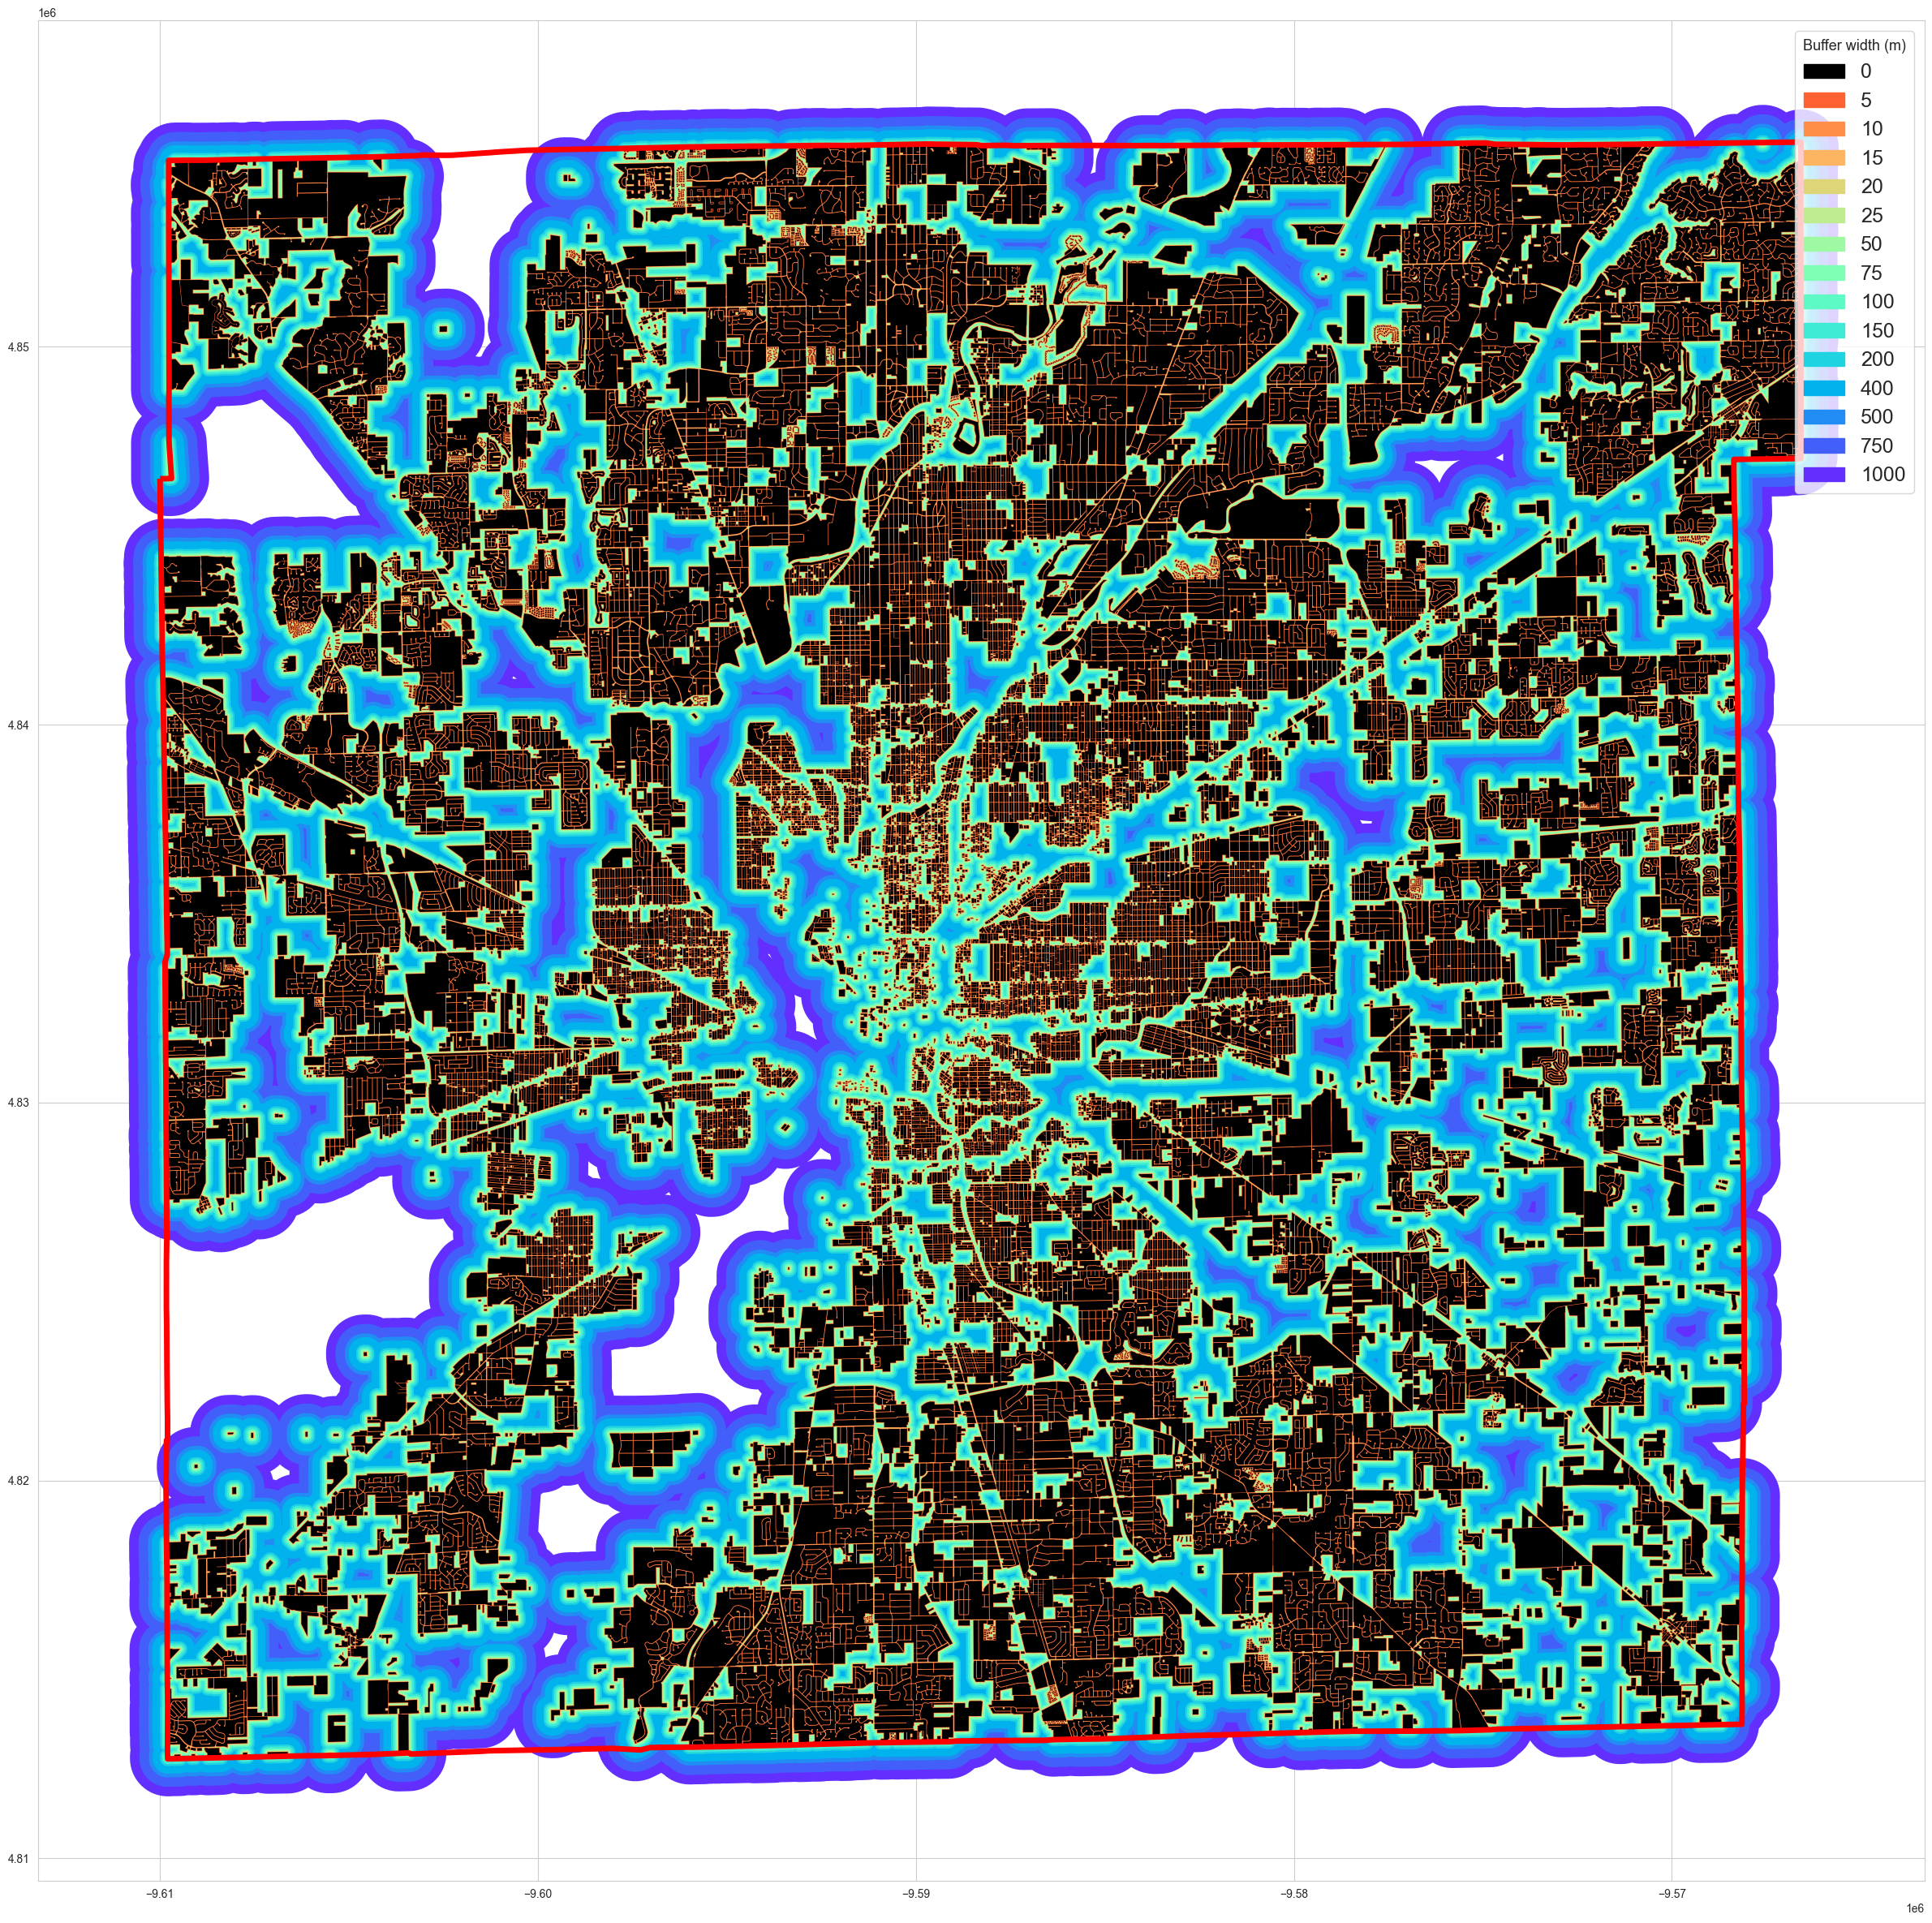
\includegraphics[width=0.8\textwidth]{figures/Indianapolis residential buffers.png}
    \caption{Indianapolis residential buffers}
    \label{fig:my_label3}
\end{figure}

\subsubsection{Proximity to home-based trips}

\begin{equation}
    \gamma(A) = \frac{1}{M} \sum_{j=1}^M \left[ \min_{k\in\{\text{orig},\text{dest}\}} \lVert \mathbf{x}_{i_j}^{\text{home}} - \mathbf{x}_j^k \rVert_2 \right]
\end{equation}

Here, $M$ is the total number of trips across all days, $i_j$ is $i^{th}$ user's $j^{th}$ trip.

\section{Results}

% Key things to ask
% \begin{enumerate}
%     \item What did we want to achieve in this study?
%     \item What methods and performance metrics did we use? How are they justified?
%     \item Which method works out the best and in what cases?
%     \item How sensitive are our results w.r.t. the algorithms’ parameters?
% \end{enumerate}

\subsection{Comparison of different MPL detection algorithms}

\subsubsection{M1: Residential detection rate}

\begin{figure}[ht]
    \centering
    \includegraphics[width=\textwidth]{figures/Result - M1.png}
    \caption{Caption}
    \label{fig:my_label}
\end{figure}

\subsubsection{M2: Proximity to trajectory}


\subsubsection{M3: Proximity to trips}

\subsection{Impact to scientific results}

\section{Discussion}
%  Which method works out the best and in what cases?
%  How sensitive are our results w.r.t. the algorithms’ parameters?
%  Sell the mobikit here.
\section*{Acknowledgments}

\section*{Author contributions}

\section*{Competing interests}
The authors declare no competing interests.

\section*{Additional information}
Supplementary Information is available for this paper.

\bibliography{bibiliography}

\end{document}
